\begin{figure}[bth!]
 \begin{center}
	\makebox[\textwidth][c]{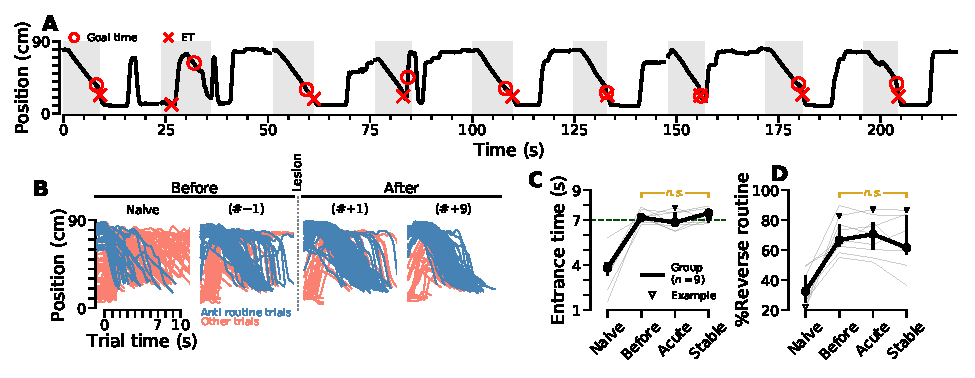
\includegraphics[scale=1]{ch-lesion/figures/ReverseTreadmill.pdf}}
	\caption[Preserved Motor Routine Performance After Lesion]
	{\textbf{Preserved performance of the run-and-wait routine following striatal lesion.}
	\textbf{(A)} Trajectory of a proficient animal trained in a version of the timing task in which the belt moved toward the reward area (rather than away from it). 9 consecutive trials and intertrials are shown.
	\textbf{(B)} Trajectories from a single representative animal in two sessions before and two sessions after lesion.
	\textbf{(C-D)} Comparison of ET (C) and percentage of run-and-wait routine usage (D), before and after striatal lesion.
	}
	\label{fig:lesion:rev}
 \end{center}
\end{figure}